%\documentclass[wsdraft]{ws-procs11x85}

\documentclass{ws-procs11x85}
\usepackage{ws-procs-thm}  
%\usepackage[demo]{graphicx}
%\usepackage{caption}
%\usepackage{subcaption}
\usepackage[caption=false]{subfig}

\begin{document}

%\title{GeneDive: A Web-based gene-gene interaction search and discovery tool}
\title{GeneDive: A gene interaction search and visualization tool to facilitate precision medicine}

\author{Paul Previde$^1$, Brook Thomas$^1$, Mike Wong$^2$, Emily K Mallory$^3$, Dragutin Petkovic$^{12}$, Russ~B~Altman$^{456}$, Anagha Kulkarni$^1$\footnote{To whom correspondence should be addressed.} \linebreak} 


\address{$^1$Department of Computer Science\\
$^2$Center for Computing for Life Sciences\\
San Francisco State University\\
San Francisco, California 94132, U.S.A. \\
E-mail: \{pprevide,bthomas\}@mail.sfsu.edu, \{mikewong, petkovic, ak\}@sfsu.edu}%\\
%www.university\_name.edu}

%\author{Emily Mallory$^1$, Russ Altman $^{234}$}
\address{$^3$Biomedical Informatics Training Program\\
$^4$Department of Bioengineering,\\
$^5$Department of Genetics,\\
$^6$School of Medicine,\\
Stanford University,\\
Stanford, California 94305, U.S.A. \\
E-mail: \{emily.mallory,russ.altman\}@stanford.edu}

\begin{abstract}
Obtaining relevant information about gene interactions is critical for understanding disease processes and treatment. With the rise in text mining approaches, the volume of such biomedical data is rapidly increasing, thereby creating a new problem for the users of this data: information overload. A tool for efficient querying and visualization of biomedical data that helps researchers understand the underlying biological mechanisms for diseases and drug responses, and ultimately helps patients, is sorely needed. To this end we have developed \emph{GeneDive}, a web-based information retrieval, filtering, and visualization tool for large volumes of gene interaction data. GeneDive offers various features and modalities that guide the user through the search process to efficiently reach the information of their interest. GeneDive currently processes over three million gene-gene interactions with response times within a few seconds.  For over half of the curated gene sets sourced from four prominent databases, more than 80\% of the gene set members are recovered by GeneDive.  In the near future, GeneDive will seamlessly accommodate other interaction types, such as gene-drug and gene-disease interactions, thus enabling full exploration of topics such as precision medicine. The GeneDive application and information about its underlying system architecture are available at http://www.genedive.net. 
\end{abstract}

\keywords{Gene Interactions; Retrieval and Visualization; Gene Sets; Gene Networks.}

% required
\copyrightinfo{\copyright\ 2017 The Authors. Open Access chapter published by World Scientific Publishing Company and distributed under the terms of the Creative Commons Attribution Non-Commercial (CC BY-NC) 4.0 License.}

% required
\bodymatter

\section{Introduction}
\label{sec:introduction}
A complete and accurate database of gene interactions (GI) is needed to understand cellular processes, disease states, and drug responses. Compiling such a database manually is a labor-intensive task, requiring highly-trained curators to identify each gene interaction and assess the quality of the supporting evidence. This approach is expensive both in time and in effort. Consequently, database curators have to limit scope by starting with key genes, drugs, or literature central to a given pathology or species of interest. This focus leads to curation bias towards well-studied or high-impact work but may miss important relationships that are not well-studied. Modern data mining techniques can scale to meet the challenge, and are automating the process of extracting interactions from biomedical literature \cite{Tari2010,Vazquez2011,Percha2012,Poon2015,em2016,Davis2017}. However, the volume of extracted data is large, and the quality is mixed.  These extracted interactions must thus be made accessible to curators and researchers in such a way as to facilitate analysis, curation, exploration, and discovery of well-understood and poorly-understood disease mechanisms and drug responses and, ultimately, to inform and improve patient care.

Current GI curation tools such as Cytoscape\cite{Shannon2003} and VisANT\cite{Hu2004} have multi-species support for integrating and visualizing curated datasets (\textit{e.g.}, GO, KEGG pathways). Literome\cite{Poon2014} uses natural language processing techniques to identify and display GIs extracted from literature. Literome provides excerpts from supporting literature, so curators can assess and vote on the interaction accuracy. However, these tools lack other features that curators find useful. To mitigate curation bias, curators need to be able to to identify GIs that are not well-studied. To our knowledge, no current tool offers an automated solution to meet this need. Another feature helpful to curators is the ability to investigate local topologies of GI networks around a gene of interest. Cytoscape and VisAnt offer comprehensive visualization, interaction selection and network analysis, while Literome has more rudimentary features.

To address the challenges of curation bias and provide needed network analysis features, we introduce GeneDive, a web-based information retrieval, filtering, topology discovery, and visualization tool that is designed to process millions of interactions efficiently. GeneDive users can sift through large volumes of data and zoom in onto a small subset of interactions of their interest. GeneDive's graphical rendering leverages Cytoscape's comprehensive visualization library, which is already familiar to many users. 

GeneDive is currently powered by a repository of over three million gene-gene interactions (GGIs) extracted using DeepDive, a scalable text-mining system~\cite{deepdive}.  The interactions were extracted from a corpus consisting of 100,000 PLOS articles and 340,000 PMC articles, and training data was extracted from BioGRID, ChEA, and Negatome~\cite{em2016}. Each extracted GGI includes an article excerpt that mentions a gene pair, and a computed probability that the relation is a true interaction. GGIs with probability of 0.9 or higher are typically true positive interactions. GGIs with slightly lower probabilities are likely to be true interactions that lack strong evidence in literature. In general, these marginal probabilities provide a unique mechanism to quickly identify poorly-studied but important GIs. GeneDive also provides other supporting evidence, such as the excerpt text, the number of instances extracted for a given GGI, and number of articles that mention the GGI.

In the near future, GeneDive's capabilities will be expanded beyond GGIs to include gene-drug and gene-disease interactions. Such a comprehensive and large repository of gene interactions can help unlock previously poorly-understood disease mechanisms and drug responses. Overall, GeneDive is designed to facilitate data-driven discovery and hypothesis testing for precision medicine researchers.

%Section~\ref{sec:genedive} introduces GeneDive and its various features.  A side-by-side feature comparison of above tools with GeneDive is also presented in Section~\ref{sec:genedive}.  The use cases in Section~\ref{sec:usecases} provide a concrete illustration of three primary use cases of GeneDive. Section~\ref{sec:recall} evaluates GeneDive's ability to recover curated gene sets, and the conclusions we draw from this work are described in Section~\ref{sec:conclusions}.



\section{GeneDive}
\label{sec:genedive}
GeneDive was developed using the agile software development approach,~\cite{agile} which entails iterative development by a cross-functional team consisting of computer scientists, developers, biomedical researchers and curators. The high-level goal was to design and develop an easy-to-use and scalable web application with powerful search functionality and multi-modal result presentation capabilities. The resulting web application and its features are described next.

\begin{figure}
\centering
\subfloat[Search input with auto-complete]{\includegraphics[width=5.3cm]{typeahead_revised.png}}\quad
\subfloat[Ambiguity resolution interface]{\includegraphics[width=5.3cm]{disambiguation.png}}\quad
\subfloat[Available search modalities]{\includegraphics[width=5.3cm]{search_modes_revised.png}}
\caption{GeneDive search entry screenshots.}
\label{fig:search}
\end{figure}

\noindent \textbf{Ambiguity Resolution:} GeneDive users can search the interactions database by entering one or more gene symbols (from Entrez/NCBI) or gene set names (from Reactome, KEGG and many others). Figure 1(a) provides an illustration of search input entry. Gene symbols are sometimes ambiguous: for example, PSP-A may refer to either of two genes, SFTPA-1 and SFTPA-2, that encode distinct pulmonary surfactant proteins. In this case, information about the genes is provided, and the user is prompted to choose the intended gene (Figure 1(b)). All gene symbol ambiguities, if any, have to be resolved before proceeding. \newline

\noindent \textbf{Topology Search:} GeneDive provides four search modes to help users investigate the GGI non-directional network topology: 1-hop, 2-hop, 3-hop, and Clique, as shown in Figure 1(c). The default mode is 1-hop, which searches for immediate neighbors, that is, genes that interact directly with the gene of interest. 1-hop retrieves all neighbors for a single-gene search, and pairwise GGIs for searches of two or more genes. For example, if the user has entered genes \emph{A}, \emph{B}, and \emph{C}, then 1-hop search will return GGIs for the following gene pairs: \emph{AB}, \emph{AC}, and \emph{BC}. 2-hop and 3-hop search modes require at least two gene symbols as input and retrieve intermediary genes along a pathway. 2-hop shows paths with one or no intermediaries, and 3-hop shows paths with two or fewer genes between the genes of interest. The intermediate genes revealed in 2-hop, 3-hop, and Clique search modes may refine our understanding of a pathway or discover new pathways. Clique search mode accepts only one gene symbol, and retrieves all the \emph{complete networks} that contain the input gene. A complete network is formed when every member gene directly interacts with every other gene in the network. 

\begin{figure}
\centerline{
    \includegraphics[width=16.5cm]{gata6_filtering_highlighting_cytoscape_revised.png}
}
\caption{Tabular (top) and graphical (bottom) views of GGIs. (Search \& controls panel on left.)}
\label{fig:results}
\end{figure}

\noindent \textbf{Graphical and Tabular Views:} Search results are presented in both tabular and graphical views, shown simultaneously and in parallel. Figure~\ref{fig:results} shows a representative view of the results of a search for gene GATA6 in the Clique mode. Users may choose to view the resulting interactions grouped by gene pairs (default) or by articles. Grouping by gene pairs collates all GGIs for every unique gene-gene pair in the retrieved results into a single row in the Table view. The \emph{Interactions} column specifies the number of GGI mentions over all articles. The number of unique articles from which these mentions are extracted is specified under \emph{Articles}. A histogram of the probabilities for the interaction group is shown in the \emph{P. Distribution} column, with the highest value shown in \emph{Max Probability}. The source sentence from which the highest-probability GGI mention was extracted is shown in the \emph{Sample Excerpt} column. 
% This presents curators with their search results, ranked by probability, as (1) GGIs; or (2) articles with GGI summaries; users can then choose to investigate a GGI, or a publication that catches their interest.

Grouped rows may be expanded to show individual interactions, each with a probability, extracted excerpt, name and hyperlink to the source article, and relevant section from the article. Nearly all of the columns are sortable in both the grouped and expanded views of the table, with descending probability as the default sort order. Gene mentions are color-coded by set membership; genes that belong to multiple sets are displayed in multiple colors. Color-coding is consistent between the graph and table views. The lower panel presents the search results in a graphical format using Cytoscape's force-directed layout engine, with nodes representing genes and edges representing interactions; edge thickness is proportional to the number of mentions for retrieved GGIs. Users can modify or change their search inputs by clicking on a node to search for that gene, or shift-clicking on one or more nodes to search for multiple genes. This allows for easy navigation of the gene interaction network. \newline

\noindent \textbf{Results Filtering and Highlighting:} The user may filter the search results using filters for one or more of the following: gene name, journal, specific article, document section (\textit{e.g.}, abstract, methods, results), excerpt partial text matching, and minimum probability cutoff (the default cutoff is 0.7). Figure~\ref{fig:results} shows the filter controls in the left panel and illustrates the negation filter: interactions containing \emph{DKK1} as one of the genes will not be retrieved.  The filters are additive; users can add or remove filters as desired. Users can highlight interactions in both views, calling attention to interactions that match the user-provided criteria (\textit{e.g.}, excerpts containing specific terms). In the graphical view, edges that match the highlighting criteria are rendered with a highlight color; in the tabular view, matching rows are also highlighted in the same color. Figure~\ref{fig:results} demonstrates highlighting for the term \emph{lysates}. For example, the first row, \emph{GATA4} and \emph{GATA6}, is highlighted because at least one of the excerpts in that group contains the term \emph{lysates}. The edge between the nodes for \emph{GATA4} and \emph{GATA6} is also highlighted in the graphical view. 

\begin{figure}
\centerline{
    \includegraphics[width=16.5cm]{genedive-architecture.png}
}
\caption{GeneDive architecture diagram showing data sources and workflow.}
\label{fig:architecture}
\end{figure}


\noindent \textbf{Saving Results:} GeneDive saves the system state; search, filter,  and highlight parameters and results; graphical views; and table contents as a state file, which can be re-uploaded to resume where the user stopped during a prior session. Tabular views can be exported to Excel. Graphical views can be saved in scalable vector graphics (SVG) format, providing users with publication-ready images of interaction networks. \newline

%\subsection{System Architecture} 
\noindent \textbf{2.1  System Architecture} \newline
\noindent GeneDive is a single-page web application following the model-view-controller (MVC) architecture. User account management and web services are implemented in PHP. As shown in Figure~\ref{fig:architecture}, the web service comprises a RESTful API layer to a SQLite relational database containing complete interaction and gene data, extracted from Entrez/NCBI, Reactome, KEGG, and DeepDive-identified GGI data. All gene references are mapped to Entrez gene IDs, and all gene sets are filtered using the GGI data; if a gene in a set does not have a DeepDive-identified interaction with any other gene in the same set, that gene is removed from the set. To improve responsiveness, most of the processing is done client-side through modules connected in serial, assisted by cached lookup tables. The modules manage filtering, coloring, synonym tagging, highlighting, grouping, and view rendering. Compressed caches include a GGI adjacency matrix with probabilities, and gene and gene set lookup tables for auto-complete. \newline

%\subsection{Feature Comparison}
\noindent \textbf{2.2 Feature Comparison with Other Tools} \newline 
\noindent Table~\ref{tab:features} provides a side-by-side comparison of GeneDive features with those of three other widely-used search and/or visualization tools: Literome, Cytoscape, and VisANT, all of which were discussed in Section~\ref{sec:introduction}.  This comparison considers 12 different features, such as whether the tool provides supporting evidence in the form of the excerpt from which the GGI was extracted, or whether the tool can search for GGIs associated with a known pathway, or whether it can support various levels of gene network analysis. As shown in Table~\ref{tab:features}, GeneDive supports more features than any of the other tools. GeneDive provides features that are traditionally supported by manually-curated databases as well as features typical of an automated database created using data mining.  

\begin{table}[ht]
\caption{Table 1.  Feature matrix of gene interaction visualization tools.}
\centering
Table 1.  Feature matrix of gene interaction visualization tools.
\label{tab:features}
\begin{tabular}{llllll}
\hline
Feature & GeneDive & Literome & Cytoscape & VisANT \\ \hline
GGI Probability               & \checkmark                    &                               &                                &                             \\
GGI Description               &                               & \checkmark                    &                                &                             \\
Supporting Literature Excerpt & \checkmark                    & \checkmark                    &                                &                             \\
KEGG Pathways                 & \checkmark                    &                               & \checkmark                     & \checkmark                   \\
Reactome Pathways             & \checkmark                    &                               & \checkmark                     & \checkmark                   \\
GO Term Enrichment            &                               &                               & \checkmark                     & \checkmark                   \\
Tabular View                  & \checkmark                    & \checkmark                    & \checkmark                     &                             \\
Graphical View                & \checkmark                    &                               & \checkmark                     & \checkmark                   \\
Direct GGI (1-hop)            & \checkmark                    & \checkmark                    & \checkmark                     & \checkmark                 \\
Intermediate GGI (2-hop)      & \checkmark                    & \checkmark                    & \checkmark                     & \checkmark                 \\
2 Intermediates (3-hop)       & \checkmark                    &                               & \checkmark                     & \checkmark                  \\
Clique                        & \checkmark                    &                               & \checkmark                     & \checkmark 				\\ \hline

\end{tabular}

\end{table}

\section{Prominent Use Cases of GeneDive}
\label{sec:usecases}

The following use cases demonstrate the features and benefits of GeneDive for research and biomedical literature curation: single-gene searches, multi-gene searches, and searches involving related genes (gene sets or pathways). \newline

\noindent \textbf{Use Case 1: Single-Gene Query.}  To demonstrate GeneDive's features and capabilities for a single-gene search, we queried the system for interactions with the gene NOD2. NOD2 is involved in immune system pathways and is associated with Crohn's disease~\cite{Yamamoto2009}.  We input NOD2 in the search bar and limited the results to probability greater than 0.80. In the gene pair group view, the result table contained interactions between NOD2 and 17 other genes. Each individual gene pair result row displayed the highest-scoring sentence for the given pair. By expanding an interaction row with a single gene, a user can display and browse supporting evidence for the interaction. For example, a user can select the row with RIPK2 and read eleven sentences that support the interaction from two different articles. In addition, the user can filter the results by specific article sections if they are more interested in sentence evidence from abstracts or results and discussion. The user also has the option to switch to the article group view in order to review all sentences with interactions from individual articles at once. This feature can hasten full-article curation. Using the gene pair group view, we discovered genes related to immune response (RIPK2~\cite{Ruefli2004}, TRAF6~\cite{Manna2005}, DUOX2~\cite{Joo2012}). After uncovering genes potentially related to the underlying mechanism for Crohn's disease, a user can query the resulting genes and construct networks with their associations. This example highlights the utility of single-gene searches for understanding the underlying mechanisms of a disease. \newline

\noindent \textbf{Use Case 2: Multi-Gene Query.}  Given a group of disease-associated genes, we would like to discover potential connections between the genes in the query set or between their interacting genes. For this example, we focused on genes related to follicular lymphoma. Translocation and subsequent overexpression of BCL2 is found in follicular lymphoma~\cite{Kridel2012}, but an additional seven genes (EZH2, ARID1A, MEF2B, EP300, FOXO1, CREBBP, and CARD11) are used for predicting disease risk~\cite{Pastore2015}.  We queried the system using their official symbols for the seven risk genes. When entering MEF2B in the search bar, a response box is triggered, requesting the user to resolve an ambiguous symbol. In this case, MEF2B is a symbol for MEF2B and BORC28-MEF2B. For the seven genes, GeneDive returned one sentence for CREBBP and EP300 as evidence for an interaction. This sentence described their individual interactions with a third gene, c-Myb, but not between themselves. Next we investigated whether any of the risk genes had interactions three or less hops (\textit{i.e.}, 3-hop) from the known causative gene BCL2. Using a probability cutoff of 0.80, we discovered four risk genes connected to BCL2 via a 3-hop search (EZH2, EP300, FOXO1, CARD11). From here, users can explore the intermediate genes and any interactions with pathway gene sets included in GeneDive.

\begin{figure}
\centerline{\includegraphics[width=16.5cm]{case_study_3.png}}
\caption{Comparison of partial network overlap of two gene sets. Genes in the insulin signaling pathway set are colored blue. Genes with both colors belong to both sets.  \textbf{Left:} Genes in the Type 2 diabetes mellitus pathway are pink. \textbf{Right:} Genes in the Type 1 diabetes mellitus pathway are pink.}
%\caption{Comparison of partial network overlap of two gene sets. Genes with both colors belong to both sets. \textbf{Left:} Genes in the insulin signaling pathway are colored blue and genes in the Type 2 diabetes mellitus pathway are colored pink. \textbf{Right:} Genes in the insulin signaling pathway are colored blue and genes in the Type 1 diabetes mellitus are pink.}
\label{fig:insulinType1v2}
\end{figure}



\noindent \textbf{Use Case 3: Pathway Gene Set Query.}  
Type 2 diabetes mellitus (T2DM) is a complex disease characterized by insulin resistance, and over the last decade, a number of genetic variants have been shown to impact disease risk~\cite{DeFronzo2015}. To demonstrate GeneDive's ability to detect potential pathway overlaps with a set of disease-related genes, we queried the system for two KEGG pathways included in the MSigDB gene sets: KEGG\_TYPE\_II\_DIABETES\_MELLITUS and KEGG\_INSULIN\_SIGNALING\_PATHWAY. While a user can input a gene set of interest, we demonstrate this feature using a pre-loaded gene set for the T2DM pathway in KEGG.%(http://www.kegg.jp/).
\footnote{\url{http://www.kegg.jp}.}
From the network view (Figure~\ref{fig:insulinType1v2}, left), numerous genes and their interactions from the T2DM pathway overlap directly with the insulin signaling pathway. This contrasts with the KEGG pathway for Type 1 diabetes mellitus (T1DM) (KEGG\_TYPE\_1\_DIABETES\_MELLITUS). Here, T1DM genes interact with those from the insulin signaling pathway, but the T1DM genes are not found in the pathway itself (Figure~\ref{fig:insulinType1v2}, right). The lack of overlap between T1DM genes and the insulin signaling pathway is due to T1DM resulting from error in insulin production, not resistance~\cite{Katsarou2017}. By including pathway gene sets in GeneDive, users have the ability to not only query their own genes or gene sets of interest, but also to investigate possible disease and biological pathway associations.


\section{Recall of Curated Gene Sets} 
\label{sec:recall}

While a good user interface is helpful to speed curator efforts, the quality of the underlying data is critical. The GeneDive data currently consists of 1,312,685 GGIs extracted from 340,000 PubMed Central ("PMC") articles, and 1,322,459 GGIs extracted from 100,000 Public Library of Science ("PLOS") articles. To assess the quality of this data, we attempt to \emph{retrieve} curated gene sets using the GGI data.  For this evaluation we use the C2 sub-collection of the GSEA MSigDB dataset, which consists of 4,731 curated gene sets\footnote{\url{http://software.broadinstitute.org/gsea/msigdb/collections.jsp}.}. The retrieval efficacy of C2 gene sets from GeneDive data is evaluated using precision and recall measures, with results shown in Table 2. We count false positives (FP) as follows: for each GGI in GeneDive data, if one gene is in any C2 gene set, and the other gene is not in any C2 gene set, then the other gene is labeled as FP. If both genes in the GGI are in the same C2 gene set, then they are identified as true positives (TP); each unique gene is counted as TP only once, even if it appears in multiple sets.  If a gene in any gene set is not labeled as TP, it is labeled as a false negative (FN). Precision is calculated as $\frac{TP}{TP+FP}$, recall as $\frac{TP}{TP+FN}$, and F1 score as $\frac{2 \cdot precision \cdot recall }{ precision + recall}$.
\begin{table}[ht]
\caption{Precision, Recall, and F1 Scores for PLOS and PubMed Central corpus}
\centering
Table 2. Precision, Recall, and F1 Scores for PLOS and PMC corpora.
\label{tab:precision-recall}
\begin{tabular}{l|llll|llll}
\hline
Cutoff & PLOS: & Precision & Recall & F1 & PMC: & Precision & Recall & F1 \\ \hline
0.0 &  & 0.941 & 0.651 & 0.770 &  & 0.941 & 0.561 & 0.703 \\
0.5 &  & 0.953 & 0.521 & 0.674 &  & 0.953 & 0.460 & 0.620 \\
0.7 &  & 0.977 & 0.246 & 0.393 &  & 0.971 & 0.259 & 0.409 \\
0.9 &  & 0.985 & 0.096 & 0.175 &  & 0.983 & 0.124 & 0.220 \\ \hline
\end{tabular}
\end{table}

These numbers suggest that the GeneDive data is fairly clean but not complete in the context of C2 gene sets, so we investigate further into the sets themselves to better understand the completeness gap. 27\% of these gene sets are contributed by either the Reactome pathway database (674 gene sets contributed), the Biocarta pathway collection (217 sets), the Pathway Interaction Database (``PID", 196 sets), or the Kyoto Encyclopedia of Genes and Genomes (``KEGG", 186 sets). The remaining gene sets are from  over nine hundred other institutions and individual contributors. C2 gene sets are of highly variable size: the smallest contain 5 genes, and the largest 1,972.  The median and the mean gene set size are 39.0 and 93.2, respectively.  As a result, we bin the gene sets based on their sizes in the following analysis. For each gene set $X$ in C2, its member genes $x_1$ and $x_2$ are labeled true positives if GeneDive data contains one or more interactions between $x_1$ and $x_2$. 

\begin{figure}
\centering

\subfloat[PMC]
{\includegraphics[width=7cm]{recall_10bins_0_0cutoff_PMC.png}}\quad
\subfloat[PLOS]
{\includegraphics[width=7cm]{recall_10bins_0_0cutoff_PLOS.png}}
\caption{Gene set recall plots for 4,731 gene sets in the MSigDB C2 collection, using GGIs extracted from (a) PMC, and (b) PLOS articles. The gene sets (binned by size) are along the X-axis, and recall percentage along the Y-axis. The median recall percentage for each bin is denoted by the horizontal line in the corresponding box.}
\label{fig:0cutoff}
\end{figure}

The results for the gene set recall analysis are given in Figure~\ref{fig:0cutoff}. The left plot shows that for half of the gene sets in a bin, about 50\% or more of its members are recovered by PMC interactions.  The recall percentages with PLOS interactions are consistently higher than those with PMC.  The median recall in the first bin (size: 5 to 10 members) is the lowest for both PMC and PLOS.  %, which is counterintuitive upon first impression. Smaller gene sets have fewer members to recover, and thus should have higher recall percentage.  
The reason for this observation becomes clearer when the sources of the gene sets are factored into this analysis.  The probabilities assigned to the interactions also significantly influence gene set recall percentages. As such, the remainder of this section investigates recall percentages in the context of specific gene set sources and probability cutoffs.  

The distribution of GeneDive probability scores resembles a normal distribution. If we filter out interactions with low probability of accuracy, then at a probability cutoff of $0.5$, 563,383 interactions from PMC qualify, and 524,140 from PLOS.  At $0.7$ cutoff, only about 10\% of the original collection remains: 133,567 interactions from PMC, and 112,282 from PLOS. Predictably, in regard to matching C2 gene sets, recall percentages decrease as more data is filtered out: at $0.5$ cutoff, about 30\% to 40\% to the gene set members are recovered for half of the gene sets in the bin. At $0.7$ this drops to 10\% to 15\%.


\begin{figure}
\centering
\subfloat[PMC]{\includegraphics[width=7cm]{recall_big3_pmc05_10.png}}\quad
\subfloat[PLOS]{\includegraphics[width=7cm]{recall_big3_plos05_10.png}}
\caption{Gene set recall plots for MSigDB gene sets from Reactome, Biocarta, PID, and KEGG, with probability cutoff of 0.5, extracted from (a) PMC, and (b) PLOS collections.}
\label{fig:big3_05cutoff}
\end{figure}

\begin{figure}
\centering
\subfloat[PMC]{\includegraphics[width=7cm]{recall_big3_pmc07_10.png}}\quad
\subfloat[PLOS]{\includegraphics[width=7cm]{recall_big3_plos07_10.png}}
\caption{Gene set recall plots for MSigDB gene sets from Reactome, Biocarta, PID, and KEGG, with probability cutoff 0.7, extracted from (a) PMC, and (b) PLOS collections.}
\label{fig:big3_07cutoff}
\end{figure}

% The sources of the gene sets had significant effects on the observed gene set recall percentages. 

%First, recall percentages were consistently and significantly higher for gene sets from Reactome, PID, KEGG, and Biocarta than for the gene sets contributed by other sources.  

If we restrict the analysis to the top four gene set contributors (\textit{i.e.}, Reactome, Biocarta, PID, and KEGG), then the recall percentages, even when using only the high-quality interactions, are substantially higher than when using all the gene sets.  At 0.5 cutoff, the recall percentage for all the gene sets was 30\% to 40\%, while for the gene sets from the top four contributors it is 70\% to 75\% (Figure~\ref{fig:big3_05cutoff}).  At 0.7 cutoff, the recall percentage for the gene sets contributed by the top four sources is about 40\% (Figure~\ref{fig:big3_07cutoff}), while for all gene sets it is 10\% to 15\%. This trend also continues in a more fine-grained analysis: at probability cutoff of 0.7, across all gene set sizes, 237 gene sets have 70\% or greater recall; of those, 207 (87.3\%) are contributed by Reactome, Biocarta, PID, or KEGG.  Conversely, out of the 132 gene sets that had a recall percentage of less than 10\%, only 2 (1.5\%) are contributed by the four sources.     

The cause for this trend is illustrated next using two gene sets, one with low recall and the other with high. An exemplary six-member gene set\footnote{\url{http://software.broadinstitute.org/gsea/msigdb/geneset\_page.jsp?geneSetName=KASLER\_HDAC7\_TARGETS\_2\_UP}.} contributed by Kasler \textit{et al.} relates to the set of genes up-regulated in DO11.10 hybridoma cells by expression of HDAC7, a signal-dependent repressor of gene transcription during T-cell development.  Using either the PLOS or PMC interaction data, the recall percentage of this set is 0\% at a 0.7 probability cutoff.  Even the primary publication \cite{Kasler2007} for this gene set does not explicitly mention, by symbol or by numerical gene identifier, any of the six genes in that set.  Many other articles mention the gene set name, but the member genes are rarely mentioned.  As such, the text mining approach used to extract GIs is unable to discover any of the member genes with high confidence.

A high-recall gene set is the Reactome ethanol oxidation set. This ten-member gene set had 100\% recall at 0.7 probability cutoff with PMC interaction data.  The Reactome documentation\footnote{\url{http://www.reactome.org/content/detail/71384}.} of this gene set includes publications as early as 1949 and as recent as 2007, nearly 60 years of research. Thus, the interactions of this gene set's members are well-documented, leading to the high recall.  
%Inasmuch as DeepDive extracts GGIs from biomedical literature, the extracted interaction data serve as an indicator of the extent of publication of the gene sets.  In this work, the gene sets contributed by Reactome, KEGG, PID, and Biocarta experienced significantly greater recall percentages than other gene sets.  This finding supports a contention that the gene sets from those four sources have a greater extent of publication in biomedical literature than the msigDB gene sets contributed by other sources.
The significantly lower recall percentages associated with small gene sets (gene sets with 5-10 members) are also explained by consideration of gene set sources.  Figures~\ref{fig:big3_05cutoff} and \ref{fig:big3_07cutoff} show that recall percentage for small gene sets contributed by the top four sources is on par with recall of larger gene sets.  The smaller gene sets from other sources, however, experience close to 0\% recall.   Collectively, Reactome, Biocarta, PID, and KEGG contribute only 55 small gene sets, while all other sources contribute 379 small gene sets. %; hence, 13\% of the small gene sets were from one of those four sources.  On the other hand, those four sources contributed 28\% of all gene sets with more than ten members.  Thus, sources other than these four provided a relatively greater fraction of small gene sets.   

%The significance of the gene set sources is shown in the boxplots of Figures~\ref{fig:big3_00cutoff}-\ref{fig:big3_07cutoff}.  
%The recall of small gene sets sourced from the four aforementioned databases is more consistent with gene sets of other sizes.  Recall percentages associated with the Reactome, Biocarta, PID, and KEGG-derived gene sets are higher across all gene set sizes and all probability cutoffs for both PMC and PLOS data (Figure~\ref{fig:sources_comp}).     

% \begin{figure}
% \centering
% \subfloat[PMC]{\includegraphics[width=7cm]{big3_pmc00_10.png}}\quad
% \subfloat[PLOS]{\includegraphics[width=7cm]{big3_00_10.png}}
% \caption{Gene set recall plots for msigDB gene sets from Reactome, Biocarta, PID, and KEGG, with gene sets recovered from the GGIs with minimum probability 0.0 extracted from (a) PMC, and (b) PLOS collections.}
% \label{fig:big3_00cutoff}
% \end{figure}

% \begin{figure}
% \centerline{\includegraphics[width=8cm]{sources_comparison_graph.png}}
% \caption{Median recall percentages for PLOS and PMC data, comparing utilization of all gene sets versus restriction to gene sets from the four sources: Reactome, Biocarta, PID, and KEGG.}
% \label{fig:sources_comp}
% \end{figure}


%However, these plots suggest that the small gene sets might also be the less popular gene sets that are not mentioned in many scholarly articles.  %( Can we substantiate this hypothesis with a few examples? )  
  
 
%As a general trend, 

% , and these sources contributed between one and fifty gene sets each.
% of genes which are known, with reasonable confidence, to be related (e.g., genes in the same biological pathway or relating to the same disease state).  



%The C2 gene sets contain from 5 to 1,972 members, with median and mean gene set sizes of 39.0 and 93.3 members, respectively.  For each gene set $X$ in C2, its members are said to be \emph{recovered} by GeneDive if the GeneDive interaction data contains one or more interactions for that pair of members.   Figure~\ref{fig:0cutoff} presents box-and-whisker plots for recall percentages of the gene sets (binned by size) utilizing the complete collection of GGIs extracted from PMC (1,312,685 interactions) and PLOS (1,322,459 interactions).  

%Since GeneDive data is compiled using an automated text mining approach, false positive interactions do exist in the data. However, such interactions are typically assigned low probability score. %   Not all the interactions in GeneDive data are true interactions.  For example, genes mentioned in a list of genes in an article might get extracted as potential interactions, although the probability value assigned to such instances is typically low.  
%In Figure~\ref{fig:0_5cutoff} and Figure~\ref{fig:0_7cutoff}, 
%Thus we also conduct gene set recall analysis by filtering out low probability interactions, $p < 0.5$, and $p < 0.7$. At probability cutoff of $0.5$, 563,383 interactions from PMC qualify, and 524,140 from PLOS.  At $0.7$ cutoff, only about 10\% of the original collection remains: 133,567 interactions from PMC, and 112,282 from PLOS.  Predictably, recall percentages decrease as more data is filtered out: at $0.5$ cutoff, about 30\% to 40\% to the gene set members are recovered for half of the gene sets in the bin.  At $0.7$ this drops to 10\% to 15\%.  The decreases in recall percentages occur because more and more of the interaction data is filtered before gene set recall takes place.     

%%\begin{figure}
%\centering
%\subfloat[PMC]{\includegraphics[width=7cm]%{10bins_0_5cutoff_PMC.png}}\quad
%\subfloat[PLOS]{\includegraphics[width=7cm]{10bins_0_5cutoff_PLOS.png}}
%\caption{Gene set Recall Plots. All gene sets.  Minimum interaction probability: $0.5$}
%\label{fig:0_5cutoff}
%\end{figure}

%\begin{figure}
%\centering
%\subfloat[PMC]{\includegraphics[width=7cm]{10bins_0_7cutoff_PMC.png}}\quad
%\subfloat[PLOS]{\includegraphics[width=7cm]{10bins_0_7cutoff_PLOS.png}}
%\caption{Gene set Recall Plots. All gene sets.  Minimum interaction probability: $0.7$}
%\label{fig:0_7cutoff}
%\end{figure}

%One of the key benefits of GeneDive is that the probability filter allows users who are specifically interested in only the highest-quality interactions (e.g., biomedical literature curators) to set the probability floor at a very high level, such as $0.9$.  At that probability minimum, 0.8\% (10,388) of the PLOS interactions and 1.3\% (16,410) of the PMC interactions qualify.  As such, the probability filter can be utilized to focus a user's attention on a very small subset of the interaction data that has the highest likelihood of representing true interactions.

\section{Conclusions}
\label{sec:conclusions}

We have developed GeneDive, a web application facilitating efficient retrieval and exploration of a large number of gene interactions. GeneDive can reveal direct and indirect relationships between two or more genes in both tabular and graphical views. Since every interaction has a confidence score (probability) and an excerpt from a cited article, the user can easily collate evidence to support or refute the hypothesis being tested. GeneDive has been designed and developed in a data-agnostic fashion so as to seamlessly process different types of interactions. Gene-drug and gene-disease interactions are slated to be integrated in GeneDive soon, making GeneDive a powerful tool for precision medicine researchers that facilitates better understanding of genetic contributions to disease and treatment outcomes.

% them to the evidence they need efficiently and easily. 

 % to refine a central database of gene interactions, and for 
 
% Furthermore, such  The GeneDive provides the probability and the excerpt  visualization formats offer powerful investigative tool for making future discoveries from the repository of GGIs.  The

%  tool helps researchers analyze the wealth of GGI information extracted from the biomedical literature by Stanford's DeepDive system.

\section*{Funding}
This work was partially supported by NIH grant LM005652, and by Center for Computing for Life Sciences at San Francisco State University. Any opinions, findings and conclusions or recommendations expressed in this material are those of the authors and do not necessarily reflect the views of the funding agency. 

% \subsection{Figures}
% \noindent A figure is obtained with the following commands

% \begin{verbatim}
% \begin{figure}[h]
% \centerline{
% 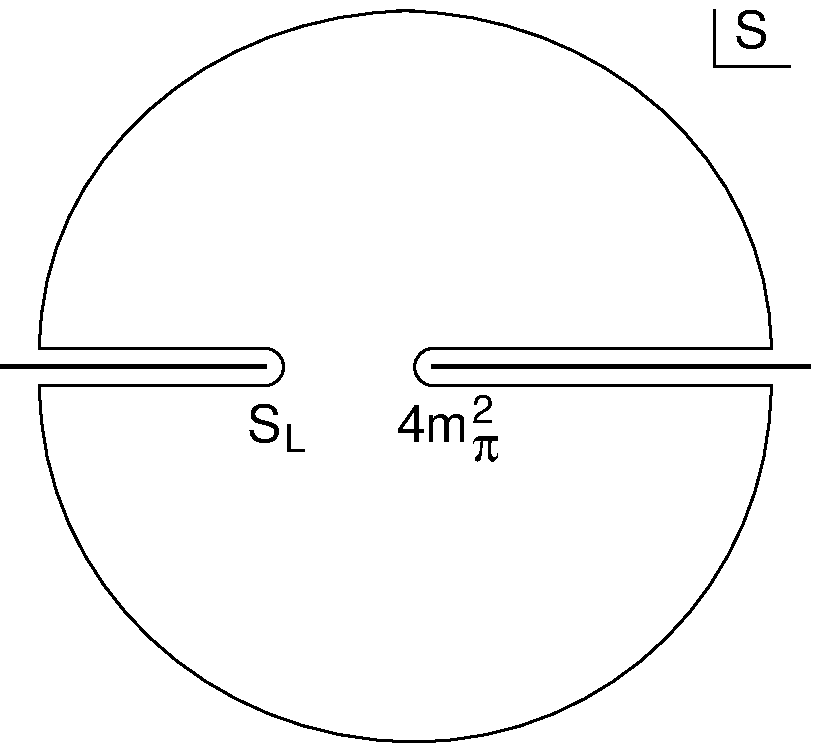
\includegraphics[width=4.5cm]{procs-fig1}
% }
% \caption{...caption here...}
% \label{aba:fig1}
% \end{figure}
% \end{verbatim}

% \begin{figure}[h]
% \centerline{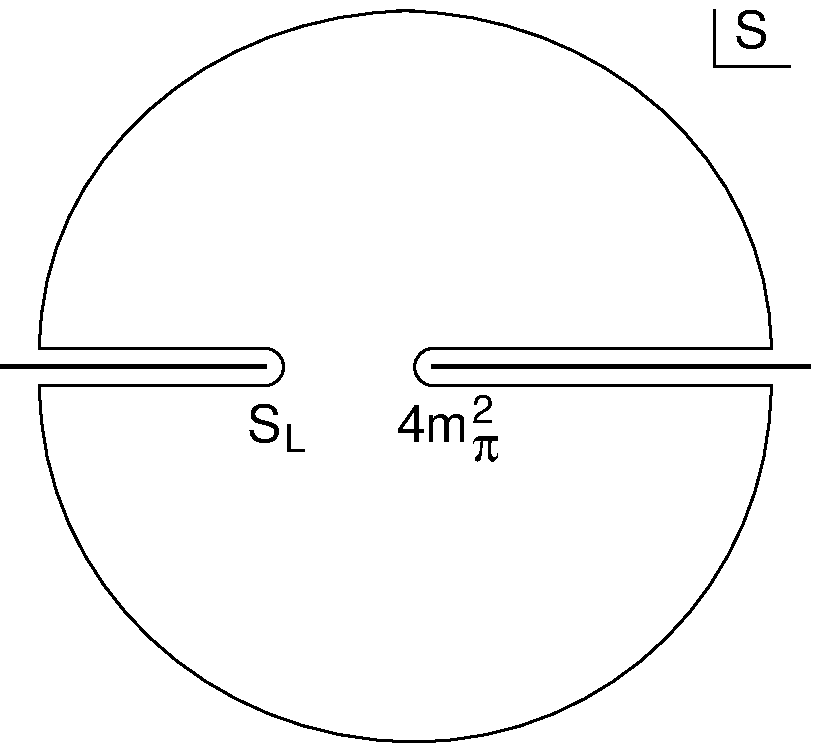
\includegraphics[width=4.5cm]{procs-fig1}}
% \caption{ ... caption here ... }
% \label{aba:fig1}
% \end{figure}

% The preferred graphics formats are TIF and Encapsulated
% PostScript (EPS) for any type of image. Our
% \TeX\ installation requires EPS, but we can easily convert TIF to EPS.
% Many other formats, e.g. PICT (Macintosh), WMF (Windows) and various proprietary
% formats, are not suitable. Even if we can read such files, there is no guarantee
% that they will look the same on our systems as on yours.

% Adjust the scaling of the figure until it is correctly positioned,
% and remove the declarations of the lines and any anomalous spacing.

% \begin{sidewaysfigure}
% \begin{center}
% 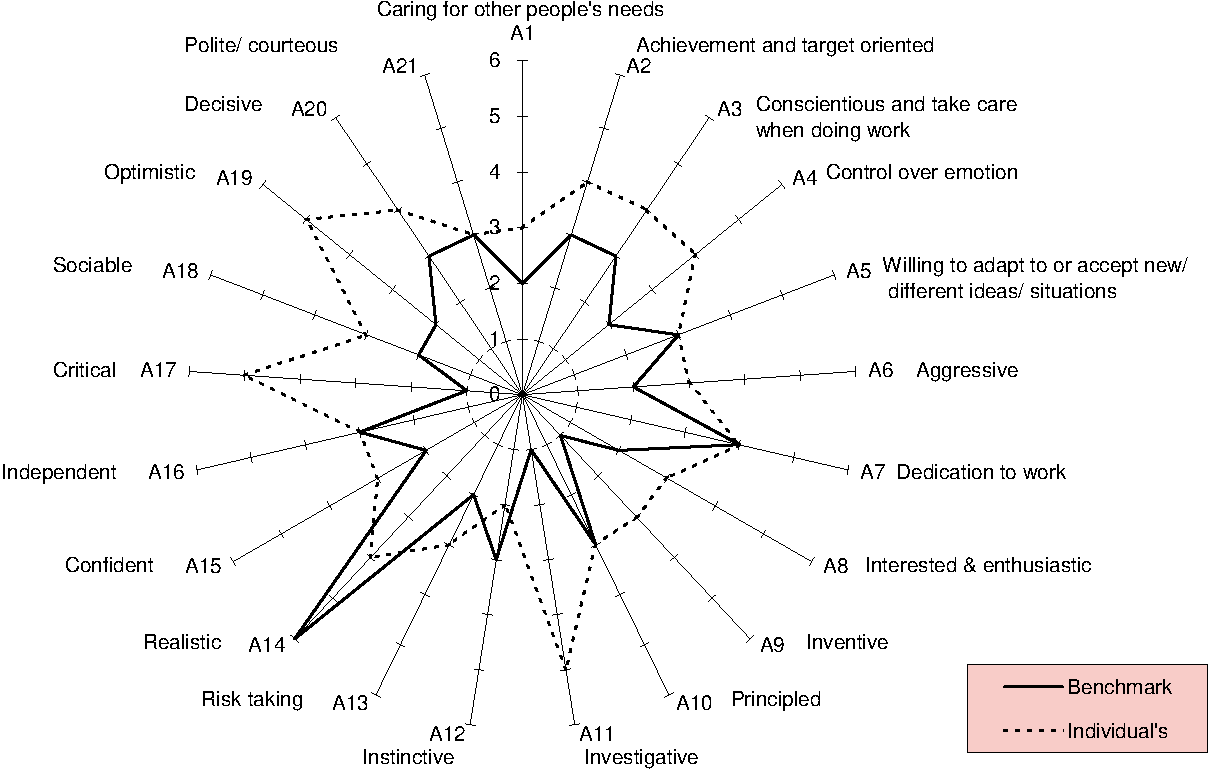
\includegraphics[width=6in]{procs-fig2}
% \end{center}
% \caption{The bifurcating response curves of system
% $\alpha=0.5$, $\beta=1.8$; $\delta=0.2$, $\gamma=0$: (a)
% $\mu=-1.3$; and\break (b) $\mu=0.3$.}
% \label{aba:fig2}
% \end{sidewaysfigure}




% Very large figures and tables should be placed on a separate page
% by themselves. Landscape tables and figures can be typeset with the following environments:
% \begin{itemize}
% \item \verb|sidewaystable| and
% \item \verb|sidewaysfigure|.
% \end{itemize}

% \noindent {\bf Example:}

% \begin{verbatim}
% \begin{sidewaysfigure}
% \begin{center}
% 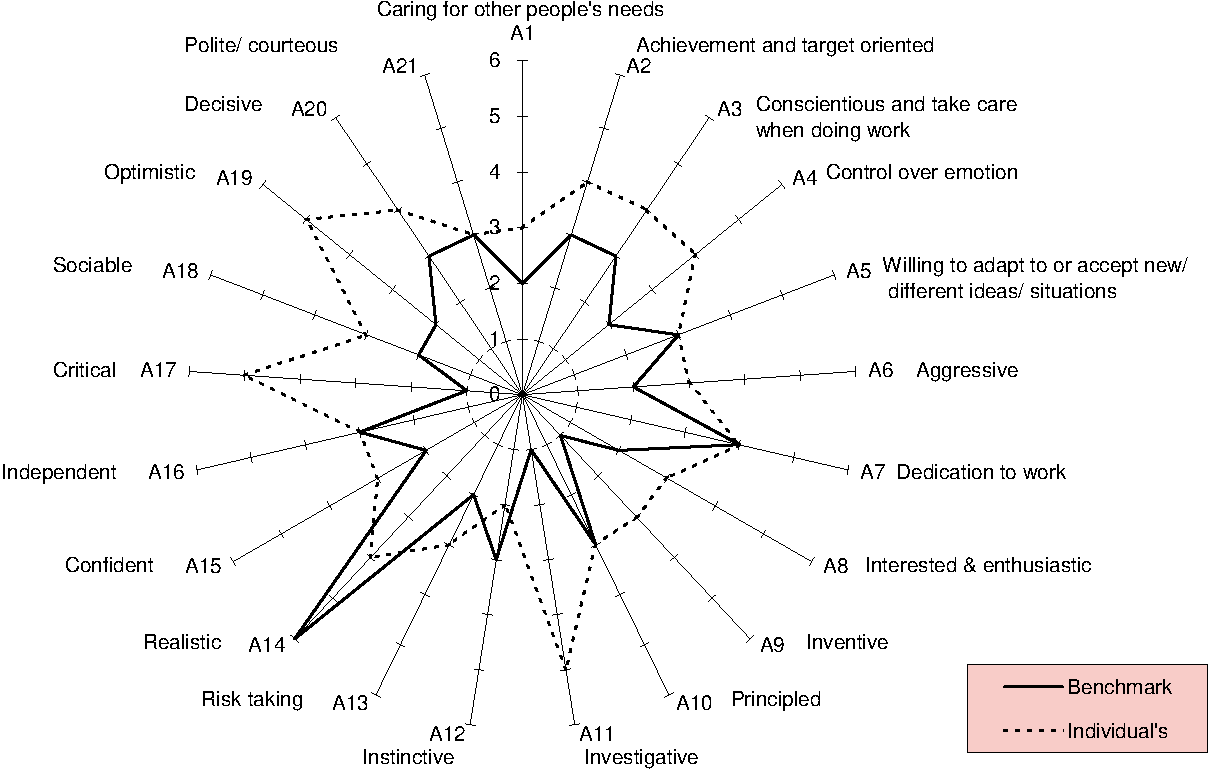
\includegraphics[width=6in]{procs-fig2}
% \end{center}
% \caption{Caption ...}
% \label{aba:fig2}
% \end{sidewaysfigure}
% \end{verbatim}

% \begin{verbatim}
% \begin{sidewaystable}
% \tbl{Positive values of ...}
% {\begin{tabular}{@{}ccccccccccc@{}}
% ...
% \end{tabular}}
% \label{aba:tbl3}
% \end{sidewaystable}
% \end{verbatim}

% \section{Cross-references}
% Use \verb|\label| and \verb|\ref| for cross-references to
% equations, figures, tables, sections, subsections, etc., instead
% of plain numbers. Every numbered part to which one wants to refer,
% should be labeled with the instruction \verb|\label|.
% For example:
% \begin{verbatim}
% \begin{equation}
% \mu(n, t) = \frac{\sum ...}{\int ...}.
% \label{aba:eq1}
% \end{equation}
% \end{verbatim}
% With the instruction \verb|\ref| one can refer to a numbered part
% that has been labeled:
% \begin{verbatim}
% ..., see also Eq. (\ref{aba:eq1})
% \end{verbatim}

% The \verb|\label| instruction should be typed
% \begin{itemize}
% \item immediately after (or one line below), but not inside the argument of
% a number-generating instruction such as \verb|\section| or \verb|\caption|, e.g.: \verb|\caption{Caption}\label{aba:fig1}|.
% \item roughly in the position where the number appears, in environments
% such as an equation,
% \item labels should be unique, e.g., equation 1 can be labeled as
% \verb|\label{aba:eq1}|, where `{\tt aba}' is author's initial and
% `{\tt eq1}' the equation number.
% \end{itemize}

% \section{Citations}
% We have used \verb|\bibitem| to produce the bibliography. Citations in the
% text use the labels defined in the bibitem declaration, e.g.,
% the first paper by Jarlskog\cite{jarl88} is cited using the command
% \verb|\cite{jarl88}|. Bibitem labels should be unique.

% For multiple citations, do not use \verb|\cite{1}|, \verb|\cite{2}|, but use
% \verb|\cite{1,2}| instead.

% When the reference forms part of the sentence, it should not
% be typed in superscripts, e.g.: ``One can show from
% Ref.~\refcite{jarl88} that $\ldots$'', ``See
% Refs.~\refcite{lamp94} and \refcite{ams04} for more details.''
% This is done using the \LaTeX{} command: ``\verb|Ref.~\refcite{name}|''.

% \section{Footnotes}
% Footnotes are denoted by a Roman letter superscript in the text. Footnotes can be used as

% \paragraph{Input:}

% \begin{verbatim}
% ... total.\footnote{Sample footnote.}
% \end{verbatim}

% \paragraph{Output:}

% \noindent ... in total.\footnote{Sample footnote text.}

% \section{Acknowledgments and Appendices}
% Acknowledgments to funding bodies etc.~may be placed in a separate
% section at the end of the text, before the Appendices. This should not
% be numbered, so use \verb|\section*{Acknowledgments}|.

% It is preferable to have no appendices in a short article, but if
% it is necessary, then simply use as

% \begin{verbatim}
% \appendix{About the Appendix}
% Appendices should be...
% \begin{equation}
% \mu(n, t) = ...
% \label{app:a1}
% \end{equation}
% \subappendix{Appendix Sectional Units}
% Sectional units are...
% \end{verbatim}

% \section{References}
% References are to be listed in the order cited in the text in Arabic
% numerals. \btex\ users, please use our bibliography style file
% \verb|ws-procs11x85.bst| for references. Non \btex\ users can list
% down their references in the following pattern.

\begin{thebibliography}{10}

\bibitem{Davis2017}  Davis AP, Wiegers TC, Roberts PM, King BL, Lay JM, Lennon-Hopkins K, Sciaky D, Johnson R, Keating H, Greene N et al. A CTD-Pfizer collaboration: manual curation of 88 000 scientific articles text mined for drug-disease and drug-phenotype interactions. Database: The Journal of Biological Databases and Curation (2013), bat080. PMC. Web. 25 May 2017.

\bibitem{DeFronzo2015}  DeFronzo RA, Ferrannini E, Groop L, Henry RR, Herman WH, Holst JJ, Hu FB, Kahn CR, Raz I, Shulman GI 
et al. Type 2 diabetes mellitus. Nature reviews Disease primers (2015), 1:15019.

\bibitem{agile} Highsmith J, Cockburn A. Agile software development: The business of innovation. Computer (2001), 34(9):120-127.

\bibitem{Hu2004} Hu Z, Mellor J, Wi J, DeLisi C. VisANT: an online visualization and analysis tool for biological interaction data. BMC Bioinformatics (2004), 5(1):17. 

\bibitem{Joo2012} Joo JH, Ryu JH, Kim CH, Kim HJ, Suh MS, Kim JO, Chung SY, Lee SN, Kim HM, Bae YS et al. Dual oxidase 2 is essential for the toll-like receptor 5-mediated inflammatory response in airway mucosa. Antioxidants \& redox signaling (2012), 16(1):57-70.

\bibitem{Katsarou2017} Katsarou A, Gudbjornsdottir S, Rawshani A, Dabelea D, Bonifacio E, Anderson BJ, Jacobsen LM, Schatz DA, Lernmark A. Type 1 diabetes mellitus. Nature reviews Disease primers (2017). %, 3:17016.

\bibitem{Kasler2007} Kasler HG, Verdin E. Histone deacetylase 7 functions as a key regulator of genes involved in both positive and negative selection of thymocytes.  Molecular and Cellular Biology (2007), 27(14). %:5184-5200. 

\bibitem{Kridel2012} Kridel R, Sehn LH, Gascoyne RD. Pathogenesis of follicular lymphoma. The Journal of clinical investigation (2012), 122(10):3424-3431.

\bibitem{em2016} Mallory EK, Zhang C, Re C, Altman RB. Large-scale extraction of gene interactions from full-text literature using DeepDive. Bioinformatics (2016), 32(1):106-113. 

\bibitem{Manna2005} Manna SK, Ramesh GT. Interleukin-8 induces nuclear transcription factor-kappaB through a TRAF6-dependent pathway. The Journal of biological chemistry (2005), 280(8):7010-7021.

\bibitem{deepdive} Niu F, Zhang C, Re C, Shavlik J.  DeepDive: Web-scale Knowledge-base Construction using Statistical Learning and Inference. VLDS, 884, 25–28.

\bibitem{Pastore2015} Pastore A, Jurinovic V, Kridel R, Hoster E, Staiger AM, Szczepanowski M, Pott C, Kopp N, Murakami M, Horn H et al. Integration of gene mutations in risk prognostication for patients receiving first-line immunochemotherapy for follicular lymphoma: a retrospective analysis of a prospective clinical trial and validation in a population-based registry. The Lancet Oncology (2015), 16(9):1111-1122.

\bibitem{Percha2012} Percha B, Garten Y, Altman RB. Discovery and explanation of drug-drug interactions via text mining. Pacific Symposium on Biocomputing. Pacific Symposium on Biocomputing (2012).%, 410-421.

\bibitem{Poon2014} Poon H, Quirk C, DeZiel C, Heckerman D; Literome: PubMed-scale genomic knowledge base in the cloud. Bioinformatics (2014), 30(19):2840-2842. 

\bibitem{Poon2015} Poon H, Toutanova K, Quirk C. Distant supervision for cancer pathway extraction from text. Pacific Symposium on Biocomputing (January 2015), 20:120–31.

\bibitem{Ruefli2004} Ruefli-Brasse AA, Lee WP, Hurst S, Dixit VM. Rip2 participates in Bcl10 signaling and T-cell receptor-mediated NF-kappaB activation. The Journal of biological chemistry (2004), 279(2). %:1570-1574.

\bibitem{Shannon2003} Shannon P, Markiel A, Ozier O, Baliga NS, Wang JT, Ramage D, Amin N, Schwikowski B, Ideker T. Cytoscape: a software environment for integrated models of biomolecular interaction networks. Genome Research, (November 2003), 13(11):2498-504

\bibitem{msigdb} Subramanian A, Tamayo A, Mootha VK, Mukherjee S, Ebert BL, Gillette MA, Paulovich A, Pomeroy SL, Golub TR, Lander ES et al. Gene set enrichment analysis: a knowledge-based approach for interpreting genome-wide expression profiles. Proceedings of the National Academy of Sciences 102.43 (2005), 15545-15550.

\bibitem{Tari2010} Tari L, Anwar S, Liang S, Cai J, Baral C. Discovering drug–drug interactions: a text-mining and reasoning approach based on properties of drug metabolism.  Bioinformatics (2010), 26(18). %:547-553, 

\bibitem{Vazquez2011} Vazquez M, Krallinger M, Leitner F, Valencia A. Text Mining for Drugs and Chemical Compounds: Methods, Tools and Applications. Molecular Informatics (June 2011), 30(6-7):506-519, 

\bibitem{Yamamoto2009} Yamamoto S, Ma X. Role of Nod2 in the development of Crohn's disease. Microbes and infection (2009), 11(12):912-918.


%\bibitem{Tari2010} C. Jarlskog, in {\it CP Violation} (World Scientific,
%   Singapore, 1988).

%\bibitem{lamp94} L. Lamport, {\it \LaTeX, A Document Preparation System},
%   2nd edition (Addison-Wesley, Reading, Massachusetts, 1994).

%\bibitem{ams04} \AmS-\LaTeX{} Version 2 User's Guide (American Mathematical
%   Society, Providence, 2004).

%\bibitem{best03} B.~W. Bestbury, {\em J. Phys. A} {\bf 36}, 1947 (2003).

\end{thebibliography}


\end{document}